\newpage

\section{Badanie ankietowe wśród pracowników branży IT}
By móc udzielić trafniejszej odpowiedzi na pytanie postawione w tytule pracy, analiza literatury została dodatkowo wsparta badaniem ankietowym przeprowadzonym wśród pracowników branży informatycznej.

\subsection{Cel badania}
Celem badania było zidentyfikowanie kluczowych kompetencji, które powinien posiadać skuteczny kierownik projektu informatycznego na podstawie dotychczasowych doświadczeń pracowników branży informatycznej. Dodatkowym aspektem tego badania w porównaniu do innych dostępnych prac było szczególne zwrócenie uwagi na umiejętności z zakresu inżynierii oprogramowania. Co pozwoliło na bardziej dokładne określienie wartości poszczególnych kompetencji technicznych i na jakim poziomie powinny być one posiadane przez kierownika projektu informatycznego. Poruszona została również kwestia szans i zagrożeń wynikających z posiadania przez kierownika projektu wiedzy technicznej.

\subsection{Metodologia oraz opis badania}
Badanie zostało przeprowadzone w formie dorbowolnej i anonimowej ankiety internetowej. Dostęp do ankiety był ograniczony, każdy z respondentów był indywidualnie zapraszany do udziału w badaniu. W badaniu wzięli udział pracownicy różnych przedsiębiorstw i poziomów organizacyjnych, co pozwoliło na uzyskanie szerokiego obrazu. 

Ankieta została podzielona na trzy sekcje. Pierwsza część dotyczyła ogólnych informacji o respondentach, takich jak ich doświadczenie zawodowe, stanowisko oraz rodzaj projektów, w których uczestniczyli. Druga część skupiła się na ocenie kompetencji kierownika projektu w różnych obszarach, takich jak umiejętności interpersonalne, przywódcze, techniczne i analityczne. W tej części ankietowani wartościowali znaczenia różnych kompetencji kierownika projektu w skali Likerta (1–5), gdzie 1 oznacza brak znaczenia, a 5 oznacza bardzo wysokie znaczenie. Ostatnia część ankiety skupiona była na aspekcie umiejętności z zakresu inżynierii oprogramowania. Oprócz pytań zamkniętych bezpośrednio nawiązujących do pytania zadanego w tytule pracy, respondenci mieli możliwość na bardziej szczegółowe wyrażenie opinii w formie pytań otwartych.
Ankieta została skonstruowana w taki sposób, aby umożliwić respondentom ocenę zarówno kompetencji technicznych, jak i miękkich. W szczególności zwrócono uwagę na umiejętności związane z inżynierią oprogramowania, które są kluczowe w kontekście zarządzania projektami informatycznymi.
Badanie zostało zrealizowane w formie anonimowej ankiety internetowej. Wzięło w nim udział 30 respondentów reprezentujących różne stanowiska w sektorze IT. Kwestionariusz zawierał pytania zamknięte , a także pytania otwarte, umożliwiające rozszerzenie odpowiedzi o opinie jakościowe.

\subsection{Charakterystyka próby}

Wśród respondentów dominowali programiści (20 osób), następnie kierownicy projektów (5 osób) oraz inne role (3 osoby) i testerzy oprogramowania (2 osoby) . Większość ankietowanych jest pracownikami branży informatycznej ponad 5 lat, dzięki czemu ich odpwiedzi są wspartę dużą wiedzą empiryczną. Dodatkowo w badaniu wzięli udział pracownicy mający doświadczenie w różnych typach projektów, co pozwoliło na uzyskanie szerokiego obrazu sytuacji. Co trzeci ankietowany miał również doświadczenie na stanowisku kierowniczym, dzięki czemu posiadają oni lepsze zrozumienie zarządzania zespołem i pracą.

\begin{figure}
  \caption{Czas pracy w branży IT}
  \centering
  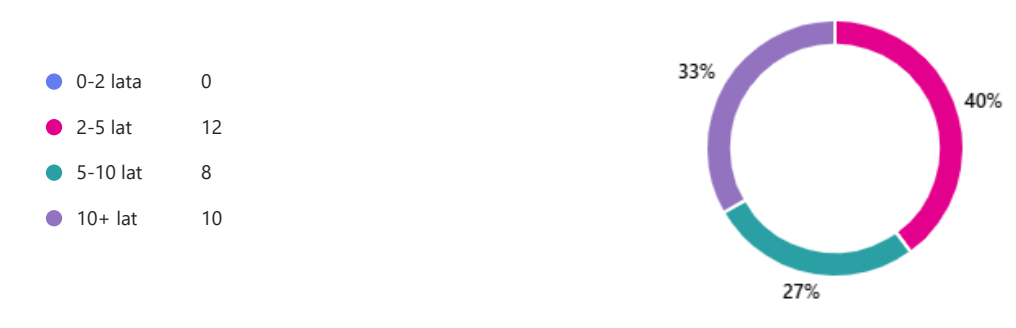
\includegraphics[width=1\linewidth]{doswiadczenie.PNG}
  \caption*{Źródło: Badanie własne}
\end{figure}

\begin{figure}
  \caption{Charakter realizowanych projektów}
  \centering
  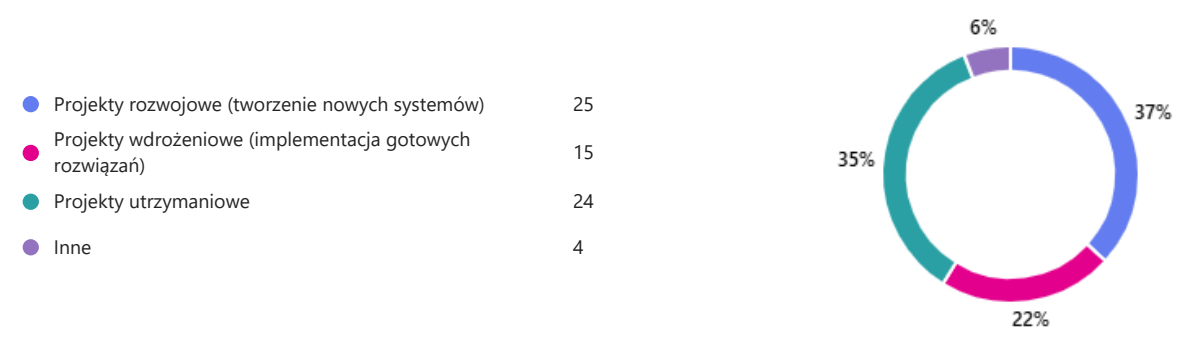
\includegraphics[width=1\linewidth]{projekty.png}
  \caption*{Źródło: Badanie własne}
\end{figure}

\subsection{Wyniki badania}

\begin{table}[htbp]
\centering
\caption{Średnie oceny kompetencji kierownika projektu IT}
\begin{tabular}{p{10cm} r}
\toprule
\textbf{Kategoria} & \textbf{Średnia / Średnia 10+} \\
\midrule
\multicolumn{2}{l}{\textbf{Kompetencje interpersonalne i komunikacyjne}} \\
Umiejętności komunikacyjne & 4{,}67 / 5{,}00 \\
Empatia i umiejętność słuchania & 4{,}23 / 4{,}20 \\
Negocjacje i rozwiązywanie konfliktów & 4{,}17 / 4{,}50 \\
\textbf{Średnia kategorii} & \textbf{4{,}36 / 4{,}57} \\  
\midrule
\multicolumn{2}{l}{\textbf{Kompetencje przywódcze i zarządcze}} \\
Przywództwo i motywowanie & 3{,}97 / 4{,}40 \\
Zarządzanie zespołem i delegowanie & 4{,}23 / 4{,}50 \\
Zarządzanie czasem i organizacja pracy & 4{,}43 / 4{,}80 \\
\textbf{Średnia kategorii} & \textbf{4{,}21 / 4{,}57} \\
\midrule
\multicolumn{2}{l}{\textbf{Kompetencje strategiczne i analityczne}} \\
Myślenie strategiczne & 4{,}17 / 4{,}10 \\
Zarządzanie ryzykiem & 4{,}17 / 4{,}20 \\
Zdolność do podejmowania decyzji & 4{,}4 / 4{,}50 \\
Znajomość i rozumienie domeny biznesowej & 4{,}07 / 4{,}20 \\
\textbf{Średnia kategorii} & \textbf{4{,}21 / 4{,}25} \\
\midrule
\multicolumn{2}{l}{\textbf{Kompetencje finansowe i organizacyjne}} \\
Zarządzanie budżetem i zasobami & 3{,}6 / 4{,}20 \\
Orientacja na wyniki i efektywność & 3{,}77 / 4{,}10 \\
Wiedza teoretyczna z zakresu zarządzania projektami & 3{,}1 / 3{,}50 \\
\textbf{Średnia kategorii} & \textbf{3{,}49 / 3{,}93} \\
\midrule
\multicolumn{2}{l}{\textbf{Kompetencje personalne}} \\
Odporność na stres & 3{,}83 / 4{,}20 \\
Cierpliwość & 3{,}9 / 4{,}20 \\
Chęć rozwoju i uczenia się & 3{,}3 / 3{,}90 \\
\textbf{Średnia kategorii} & \textbf{3{,}68 / 4{,}10} \\
\midrule
\multicolumn{2}{l}{\textbf{Kompetencje z zakresu inżynierii oprogramowania}} \\
Formułowanie wymagań dotyczących oprogramowania & 3{,}57 / 3{,}30 \\
Metody testowania i weryfikacji poprawności & 2{,}73 / 2{,}50 \\
Znajomość cyklu życia systemów informatycznych & 2{,}5 / 3{,}90 \\
Znajomość wzorców projektowych i architektonicznych & 2{,}15 / 2{,}40 \\
Umiejętność programowania & 2{,}17 / 2{,}00 \\
Wiedza w zakresie baz danych & 2{,}27 / 1{,}90 \\
Wiedza w zakresie algorytmów i struktur danych & 1{,}93 / 2{,}00 \\
Znajomość systemów operacyjnych, sieci komputerowych i bezpieczeństwa & 2{,}17 / 2{,}30 \\
\textbf{Średnia kategorii} & \textbf{2{,}67 / 2{,}54} \\
\bottomrule
\end{tabular}
\caption*{Średnia – średnia ocen dla wszystkich badanych; Średnia 10+ – średnia ocen dla pracowników z stażem 10 lat i więcej. Źródło: Badanie własne.}
\end{table}

\subsubsection{Porównanie średnich ocen kompetencji}

Wyniki badania pokazują, że Kategorie kompetencji interpersonalnych i przywódczych uzyskały najwyższe oceny, co potwierdza ich kluczowe znaczenie w zarządzaniu projektami IT. Dodatkowo warto zwrócić uwagę, że pracownicy z większym doświadczeniem w branży ocenili te komptencje jeszcze wyżej niż ogół. Pojedynczo najważniejszą kompetcją okazały się umiejętności komunikacyjne. Wśród pracowników ze stażem 10+ otrzymały one średnią 5.00. Następnie w kolejności z pojedynczych umiejętności znalazło się zarządzanie czasem i organizacja pracy oraz delegowanie zadań. Wyniki te sugerują role jaką według badanych powinien pełnić kierownik projektu w zespole. Powinien on być osobą, która nie tylko zarządza zespołem, ale również jest w stanie skutecznie komunikować się z jego członkami oraz motywować ich do działania. Wysoka ocena kompetencji strategicznych i analitycznych poazuje, że kierownicy projektów powinni być w stanie myśleć krytycznie i podejmować decyzje na podstawie analizy danych. szczególne wysoko w tej kategorii oceniono umiejętność podejmowania decyzji oraz zarządzanie ryzykiem. Kompetencje te są szczególnie istotne w kontekście projektów informatycznych, gdzie zmiany mogą występować w każdej chwili, a kierownik projektu musi być w stanie szybko dostosować się do nowych warunków.
Kompetencje finansowe i organizacyjne oceny poniżej 4, co sugeruje, że są one mniej istotne w kontekście zarządzania projektami IT. Jednak respondenci z większym doświadczeniem wyrażniej wyżej niż ogół ocenili rolę zarządzania budżetem i zasobami oraz orientacje na wyniki Szczególne nisko została oceniona wiedza teoretyczna z zakresu zarządzania projektami, co może sugerować, że praktyczne umiejętności i naturalne predyspozycje są bardziej cenione niż teoretyczna wiedza.
indywidualne kompetencje personalne kierownika projektu również nie uzyskały zbyt wysokiej oceny, gdyż średnia dla tej Kategorii wyniosłą poniżej 4. Warto zwrócić w tym przypadku uwagę na różnice między średnią ogólną a pracownikami bardziej doświadczonymi. Ta druga grupa zwróciła wyraźnie podkreśliła znaczenie takich cech jak cierpliwość i odporność na stres. Co może sugerować, że w miarę zdobywania doświadczenia w branży IT, respondenci zaczynają dostrzegać znaczenie tych cech w kontekście zarządzania projektami. Kształtowanie cierpliwość i odporność na stres może być kluczowe dla skutecznego zarządzania projektami, zwłaszcza w obliczu wyzwań i stresu, które często towarzyszą pracy w branży IT.
Kompetencje z zakresu inżynierii oprogramowania uzyskały najniższe oceny, co może wskazywać na ich marginalne znaczenie w kontekście kierowania projektami informatycznymi. Respondenci wskazali, że kierownik projektu nie musi być ekspertem technicznym, ale powinien mieć podstawową wiedzę na temat technologii i procesów związanych z inżynierią oprogramowania. W tej kategorii szczególnie wyróżniały się umiejętności formułowania wymagań dotyczących oprogramowania oraz znajomość cyklu życia systemów informatycznych. Bardzo duża różnica występuje w przypadku oceny znajmości cyklu życia systemów informatycznych, gdzie pracownicy z większym doświadczeniem ocenili tę umiejętność na 3{,}90, podczas gdy ogół na 2{,}50. Może to sugerować, że w celu skutecznego zarządzania projektem kierownik powinien dobrze znać cykl życia systemów informatycznych, aby móc skutecznie komunikować się z zespołem i podejmować decyzje dotyczące projektu. Warto również zauważyć, że umiejętności programowania oraz znajomość algorytmów i struktur danych uzyskały najniższe oceny, co sugeruje, że nie są one kluczowe dla kierownika projektu. Respondenci wskazali, że kierownik projektu nie musi być ekspertem technicznym, ale powinien mieć podstawową wiedzę na temat technologii a w szczególności procesów związanych z inżynierią oprogramowania.

\subsubsection{Ocena wymaganego doświadczenia technicznego kierownika projektu}
W kolejnej części badania, która skupiała się już konkretnie na ocenie znaczenia umiejętności z zakresu inżynierii oprogramowania u kierownika projektu, respondenci zostali poproszeni o wyrażenie opinii, czy kierownik projektu IT powinien posiadać praktyczne doświadczenie w inżynierii oprogramowania. Tylko 13\% odpowiedziało stanowczo, iż jest to niezbędne, 23\% respondentów oceniła praktyczne doświadczenie jako niepotrzebne. Zdecydowana większość zaś zwróciła uwagę, iż zależy to przede wszystkim od typu projektu. Ma to również potwierdzenie w przytaczanej w poprzednich rozdziałach literaturze, gdyż Nicholas i Steyn\autocite{NicholasSteyn} wyraźnie podkreślili, że wymagane umiejętności z zakresu inżynierii oprogramowania u kierownika są uwarunkowane właśnie zaawansowaniem technicznym realizowanego projektu.
Następnie respondenci, którzy odpowiedzieli na to pytanie "Tak" lub "Zależy" zostali poproszeni o ocenę poziomu umiejętności w dziedzinie inżynierii oprogramowania jakie powinien mieć kierownik projektu informatycznego. W tej części badania respondenci mieli możliwość wyrażenia swojej opinii za pomocą porównania wymaganych umiejętności do kompetencji programisty na różnych etapach kariery. Respondenci mieli do wyboru pięć poziomów, które odpowiadały poziomowi umiejętności programisty na różnych etapach kariery zawodowej. Poziomy te to: stażysta, młodszy programista, programista, starszy programista oraz architekt systemów informatycznych. Dodatkowo określona została kategoria "Porównanie nieadekwatne" w celu zapewnienia większej swobody odpowiadającym i weryfikacji ich iterpretacji umiejętności w dziedzinie inżynierii oprogramowania. Kategoria ta uzyskała stosunkowo wysoką popularność, aż pięciu odpowiadających wybrało tą odpowiedź. Co może sugerować, że biegłość techniczna u kierownika projektu nie jest tym samym co wymagane jest od programisty. Zdecydowana większość respondentów jednak wybrała opcję programista, według raporty BulldogJob średni czas doświadczenia dla programisty to 5 lat\autocite{BulldogJob}. Jest to stosunkowo długi okres i może oznaczać duży próg wejścia dla przyszłych kierowników projektów informatycznych, szczególnie w przypadku projektów zaawansowanych technicznie.

\begin{figure}
  \caption{Czy kierownik projektu IT powinien posiadać praktyczne doświadczenie w inżynierii oprogramowania?}
  \centering
  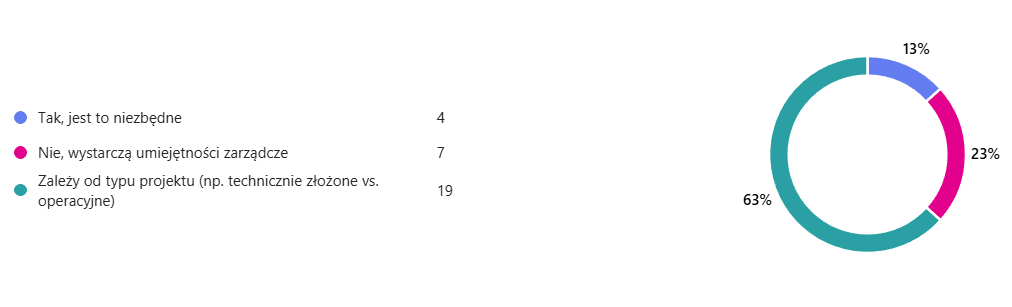
\includegraphics[width=1\linewidth]{czy_inzynier.png}
  \caption*{Źródło: Badanie własne}
\end{figure}

\begin{figure}
  \caption{Ocena poziomu umiejętności w dziedzinie inżynierii oprogramowania jakie powinien mieć kierownik projektu informatycznego}
  \centering
  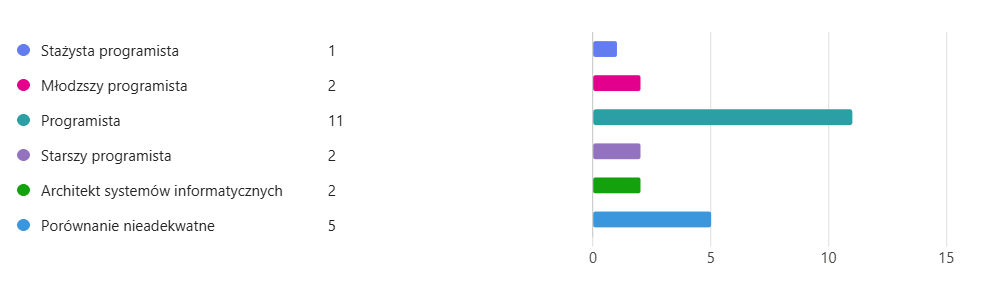
\includegraphics[width=1\linewidth]{poziom.png}
  \caption*{Źródło: Badanie własne}
\end{figure}

\begin{figure}
  \caption{Poziom doświadczenia a doświadczenie w latach}
  \centering
  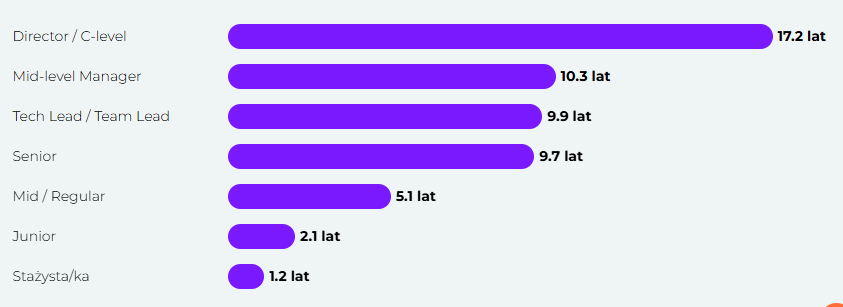
\includegraphics[width=1\linewidth]{bulldog.png}
  \caption*{Źródło: https://bulldogjob.pl/it-report/2025/programista}
\end{figure}

\subsection{Wpływ wiedzy z zakresu inżynierii oprogramowania na zarządzanie projektem informatycznym}
W następnym pytaniu ankietowani zosta poproszeni o określenie jaki według nich wpływ na poszczególne aspekty zarządzania projektem informatycznym ma wiedza z zakresu inżynierii oprogramowania. Badne były trzy składowe: efektywna komunikacja, zarządzanie ryzykiem oraz realizaja celów projektu, do oceny poszczególnych aspektów respondenci mieli do wyboru pięciostopniową skalę, gdzie 1 oznacza brak wpływu, a 5 oznacza bardzo duży wpływ. Znacząca wiekszość oceniła wpływ wiedzy z zakresu inżynierii oprogramowania na efektywną komunikację oraz zarządzanie ryzykiem na 4 lub 5. Co może sugerować, że wiedza techniczna jest istotnym czynnikiem w kontekście tych aspektów zarządzania projektem. Dużo większą rozbieżność odpowiedzi widać w przypadku oceny realizacji celów projektu, respondenci byli bardziej podzieleni, co może sugerować, że wiedza techniczna nie jest kluczowym czynnikiem wpływającym na ten aspekt zarządzania projektem.

\begin{figure}
  \caption{Wpływ wiedzy z zakresu inżynierii oprogramowania na poszczególne aspekty zarządzania projektem}
  \centering
  
\includegraphics[width=1\linewidth]{wplyw.png}
  \caption*{Źródło: Badanie własne}
\end{figure}

\begin{table}[h]
\centering
\caption{Średnie oceny wpływu wiedzy z zakresu inżynierii oprogramowania na poszczególne aspekty zarządzania projektem informatycznym}
\begin{tabular}{p{10cm} r}
\toprule
\textbf{Kategoria} & \textbf{Średnia / Średnia kierownik} \\
\midrule
Efektywna komunikacja z zespołem & 3{,}40 / 3{,}45 \\
Zarządzanie ryzykiem & 3{,}27 / 3{,}27 \\
Realizacja celów projektu & 3{,}20 / 3{,}00 \\
\textbf{Średnia wszystkich kategorii} & \textbf{3{,}29 / 3{,}24} \\  
\bottomrule
\end{tabular}
\caption*{Średnia – średnia ocen dla wszystkich badanych; Średnia kierownik – średnia ocen dla pracowników z doświadczeniem na stanowisku kierowniczym. Źródło: Badanie własne.}
\end{table}

Dodatkowo w tabeli zostało przedstawione porównanie średnich ocen dla wszystkich badanych oraz dla pracowników, którzy mieli doświadczenie na stanowiskach kierowniczych. Nie widać szczególnych różnic pomiędzy obiema grupami, osoby z doświadczeniem kierowniczym nie wydają się widzieć większego niż reszta wpływu wiedzy z zakresu inżynierii oprogramowania na wymienione aspekty zarządzania projektem informatycznym. 

\subsection{Negatywny wpływ braku wiedzy technicznej na zarządzanie projektem informatycznym}
W ostatnim pytaniu zamkniętym badani odpowadali czy doświadczyli oni negatywnego wpłwu braku wiedzy technicznej u kierownika projektu na realizację projektu. Połowa ankietowanych odpowiedziała, że "Nie", zaś pozstała część podzieliła się na dwie grupy, które odpowiedziały "Tak" oraz "Nie wiem". 

\begin{figure}
  \caption{Czy ma Pan/Pani doświadczenie sytuacji, w której brak wiedzy technicznej u kierownika projektu negatywnie wpłynął na realizację projektu?}
  \centering
  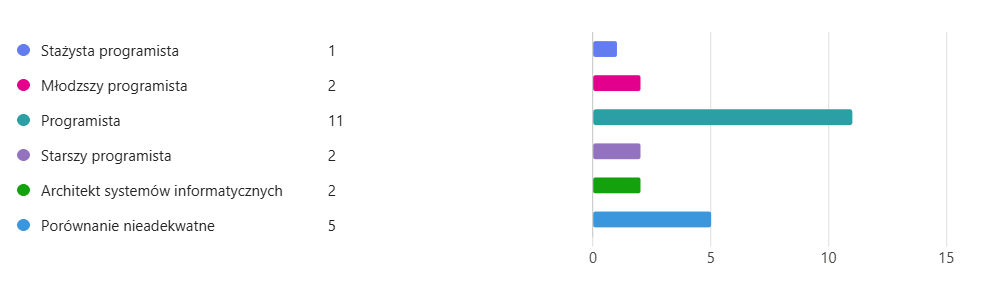
\includegraphics[width=1\linewidth]{poziom.png}
  \caption*{Źródło: Badanie własne}
\end{figure}

Dodatkowo osoby, które odpowiedziały "Tak" zostały poproszone o podanie konsekwencji, które ich zdaniem wynikły z braku wiedzy technicznej u kierownika projektu. Respondenci wskazali na następujące problemy:
\begin{itemize}
  \item wydłużenie czasu realizacji projektu, w związku ze złą wyceną czasu realizacji zadań,
  \item brak decyzyjności spowodowany strachem przed podjęciem złej decyzji i nieznajomością tematu,
  \item źle sformułowane wymagania - nieprezyjne lub niemożliwe do zrealizowania,
\end{itemize}

Warto przytoczyć również dwie odpowiedzi, które szczególnie dobrze podsumowują problem:
\begin{quote}
  \textit{Brak zrozumienia tematu przez kierownika projektu powodował, że nie chciał on się zaangażować w rozwiązywanie problemu i oczekiwał jedynie na wypracowanie rozwiązania przez inżynierów.}
\end{quote}
\begin{quote}
  \textit{Opóżnienia w realizacji projektu - np. brak sprawczosci w koordynowaniu zadań na styku wielu zespołów. Brak sprawczości na poziomie decyzyjnym/zarządu. Brak zrozumienia wartości dostarczanych przez rozwiązanie IT.}
\end{quote}


Wypowiedzi te jasno wskazują, że kierownik projektu, który nie posiada wiedzy technicznej, może mieć trudności w podejmowaniu decyzji oraz koordynowaniu działań zespołu. W rezultacie może to prowadzić do opóźnień w realizacji projektu oraz braku efektywności w zarządzaniu zespołem. 

Interesująca wydaje się również wypowiedź dotycząca outsourcingu:
\begin{quote}
  \textit{W przypadku outsourcingu lub korzystania z usług firm zewnętrznych PM może zostać łatwo oszukany przez zewnętrznego dostawcę.}
\end{quote} 

Odpowiedź ta wskazuje na wcześniej niewspomniane ryzyko związane z brakiem wiedzy technicznej u kierownika projektu. W przypadku współpracy z zewnętrznymi dostawcami, co jest powszechnym trendem w branży IT, brak technicznego zrozumienia może prowadzić do sytuacji, w której dostawca narzuca nieoptymalne lub przesadnie kosztowne rozwiązania, a kierownik projektu nie jest w stanie skutecznie weryfikować ich zasadności z biznesowego punktu widzenia.

\subsection{Zagrożenia wynikające z nadmiernego skupienia się kierownika projektu na aspektach technicznych}
Ostatnia część badania było to pytanie otwarte i dotyczyło zagrożeń wynikających z nadmiernego skupienia się kierownika projektu na aspektach technicznych. Respondenci zostali poproszeni o wskazanie, jakie problemy mogą wystąpić w przypadku, gdy kierownik projektu zbytnio koncentruje się na szczegółach technicznych. W toku badania wyłoniły się cztery główne obszary ryzyka, na które zwracali uwagę uczestnicy:

\begin{itemize}
  \item \textbf{Micromanagement i wchodzenie w kompetencje zespołu} - gdy kierownik projektu angażuje się w każdy techniczny detal, zaczyna pełnić rolę „wąskiego gardła” w procesie decyzyjnym i realizacji zadań. Zamiast delegować odpowiedzialność doświadczonym programistom lub architektom, narzuca on im własne rozwiązania, co osłabia ich motywację, podważa poczucie autonomii oraz prowadzi do zaburzeń w naturalnym przepływie informacji. Tego typu mikrozarządzanie nie tylko wydłuża czas pracy nad poszczególnymi zadaniami, ale również wprowadza konflikty kompetencyjne, gdy specjalista czuje, że jego wiedza i doświadczenie są lekceważone.
  \item \textbf{Zaniedbanie roli menedżerskiej i celów biznesowych} - skupienie na szczegółach technicznych powoduje, że kierownik traci z pola widzenia nadrzędne cele biznesowe projektu. Zamiast nadzorować postęp prac, zapewniać efektywną komunikację między interesariuszami oraz dbać o jakość dostarczanej wartości, poświęca większość czasu na analizę rozwiązań technicznych. W efekcie może dojść do rozmycia wymagań, braku spójności dokumentacji oraz stworzenia produktu, który choć technicznie dopracowany, to nie odpowiada potrzebom klienta ani strategicznym założeniom organizacji.
  \item \textbf{Ryzyko opóźnień i technicznego przeinwestowania} - zjawisko overengineeringu, czyli dążenie do idealnego rozwiązania technicznego\autocite{overengineering}, często skutkuje przeciąganiem faz implementacji. W miejsce prostego i szybkiego wdrożenia pojawiają się rozbudowane konstrukcje architektoniczne „na zapas”, które nie zawsze przekładają się na realne korzyści, a jedynie generują dodatkowe koszty i opóźnienia.
\end{itemize}

Poniżej przedstawiono kilka wypowiedzi respondentów, które ilustrują te zagrożenia:

\begin{enumerate}
  \item \emph{„Zbytnie dążenie do stworzenia idealnego technicznie systemu, co opóźnia tworzenie takiego systemu.”}  
  Ta uwaga trafnie oddaje paradoks overengineeringu: zamiast dostarczyć prosty, działający produkt, zespół wpada w spiralę ulepszeń, zagrażając terminowemu zakończeniu projektu.
  
  \item \emph{„Odklejenie od biznesu. Overengineering. Tworzenie \emph{bottleneck}’ów.”}  
  Skondensowana definicja ryzyk: micromanagement łączy się tu z utratą perspektywy biznesowej, a wąskie gardła wynikają zarówno z nadmiernego uszczegółowienia, jak i braku klarownego priorytetu na potrzeby klienta.
  
  \item \emph{„W przypadku outsourcingu lub korzystania z usług firm zewnętrznych PM może zostać łatwo oszukany przez zewnętrznego dostawcę.”}  
  Rzadziej omawiany aspekt – brak technicznej bezstronności w relacjach B2B może narazić projekt na niekorzystne zobowiązania, gdy dostawca proponuje rozwiązania trudne w niezależnej weryfikacji.
\end{enumerate}


\subsection{Wnioski}

Analiza wyników badania ankietowego wskazuje, że kluczową wartość w pracy kierownika projektu informatycznego stanowią umiejętności interpersonalne i komunikacyjne, które pozwalają na skuteczne budowanie relacji z zespołem oraz utrzymanie klarownej wymiany informacji. Równie istotne okazały się być kompetencje przywódcze i organizacyjne — zdolność motywowania, delegowania zadań oraz efektywnego zarządzania czasem i zasobami, co przekłada się na realizację założeń projektu w terminie. 

Choć techniczne kompetencje z zakresu inżynierii oprogramowania otrzymały od respondentów niższe oceny, badanie wykazało, że podstawowa wiedza na temat cyklu życia systemów, formułowania wymagań czy znajomość metod weryfikacji kodu są ważne i przydatne w roli kierownika projektu informatycznego. Ankietowani zauważyli również potencjał w wiedzy z zakresu inżynierii oprogramowania jako wsparcie efektywnej komunikacji z zespołem. Z drugiej strony jednak zbyt duże zaangażowanie kierownika w szczegóły techniczne może prowadzić do mikrozarządzania, narastania kosztów oraz opóźnień spowodowanych overengineeringiem i utratą koncentracji na celach biznesowych. 

Kierownik projektu powinien zatem znajdować złoty środek: łączyć silne kompetencje miękkie i przywódcze z kontekstową, adekwatną do stopnia skomplikowania projektu wiedzą techniczną. Dzięki takiemu zrównoważonemu podejściu możliwe jest zachowanie równowagi między sprawnym zarządzaniem zespołem a trafnym podejmowaniem decyzji biznesowych oraz rzetelną współpracą z ekspertami technicznymi.

Można więc stwierdzić, że skuteczny kierownik projektu informatycznego powinien funkcjonować jako swego rodzaju łącznik – mediator pomiędzy światem technologicznym a biznesowym, osoba, która nie tylko rozumie język kodu, ale przede wszystkim potrafi przekształcić wymagania klienta w realne działania zespołu. Tylko takie zrównoważenie kompetencji miękkich i twardych pozwala na stworzenie środowiska sprzyjającego efektywnej współpracy, minimalizacji ryzyka i dostarczaniu wartości dla interesariuszy.

Wyniki badania korespondują z ustaleniami przedstawionymi w literaturze przedmiotu, omawianej w poprzednich rozdziałach, co wzmacnia ich wiarygodność oraz potwierdza aktualność poruszanych zagadnień.